\documentclass[11pt,letterpaper]{article}

% ------------------------------------------------------------
% Packages
% ------------------------------------------------------------
\usepackage[margin=1in]{geometry}
\usepackage{graphicx}
\usepackage{subcaption}
\usepackage{booktabs}
\usepackage{amsmath,amssymb}
\usepackage{float}
\usepackage{placeins}
\usepackage{microtype}
\usepackage{xcolor}
\usepackage[hidelinks]{hyperref}

\graphicspath{{../figures/breakdown/}{../figures/}{../schematics/}}

% Shorthand macros
\newcommand{\nWr}{\ensuremath{\overline{\text{Wr}}}}
\newcommand{\Vdd}{\ensuremath{V_{DD}}}
\newcommand{\um}{\ensuremath{\,\mu\text{m}}}
\newcommand{\uW}{\ensuremath{\,\mu\text{W}}}

% ------------------------------------------------------------
% Title
% ------------------------------------------------------------
\title{\vspace{-1.5em}ESE~3700 Project~2:\\A 16$\times$4 SRAM in 22\,nm PTM HP}
\author{Lucas Krippendorff}
\date{April 2026}

\begin{document}
\maketitle

% ============================================================
\section{Introduction}
% ============================================================

This report describes the design, validation, and characterization of a
$16\times4$ single-port SRAM implemented in the 22\,nm PTM high-performance
BSIM4 process at $\Vdd=0.8$\,V. The memory provides synchronous,
full-word (4-bit) random read/write access using a 4-bit address, a single
clock, and an active-high write enable. Correct operation is demonstrated
across a suite of functional tests, and the design is characterized against
the project figure of merit
\[
  \mathrm{FOM} \;=\; 60 \cdot \mathrm{BitcellArea} \cdot P \cdot D^2,
\]
using the worst-case access delay and the average power during the specified
all-zeros/all-ones write workload. The resulting FOM is
$\mathbf{8.46\times10^{6}~\mu\text{m}\cdot\mu\text{W}\cdot\text{ps}^{2}}$
at a 320\,ps measurement period (3.125\,GHz), well above the 500\,MHz
requirement.

% ============================================================
\section{Top-Level Architecture}
% ============================================================

\begin{figure}[H]
  \centering
  
\includegraphics[width=0.92\linewidth]{main.png}
  \caption{Top-level schematic (\texttt{main}). External pins: \texttt{A0--A3},
  \texttt{Clk}, \texttt{Wr}, \texttt{bit0--bit3}. $\Vdd$/GND are handled as
  globals through each leaf cell; they are not exported on the top icon.}
  \label{fig:main}
\end{figure}

The memory is hierarchically composed of the following sub-cells, each of
which is described in Section~\ref{sec:subcomponents}:

\begin{itemize}
  \item \textbf{2PhaseClock} -- generates non-overlapping clocks
        $\phi_1$ (precharge) and $\phi_2$ (access) from the single input
        \texttt{Clk}.
  \item \textbf{Decoder4to16} -- decodes \texttt{A0--A3} and gates each row
        output with $\phi_2$ to produce one of sixteen word-lines
        $\mathrm{WL}[0..15]$.
  \item \textbf{array} -- 16 instances of \texttt{wordRow}, each containing
        four 6T \texttt{Bitcell}s sharing a common WL.
  \item \textbf{ColumnDriver} $\times 4$ -- contains the precharge PMOS pair
        (gated by \texttt{PCHb}) and a tri-stated write driver (gated by
        \texttt{Wr}).
  \item \textbf{SenseAmp} $\times 4$ -- an isolated latch-type sense amplifier
        (Section~\ref{sec:sa}).
  \item \textbf{ANDmin} + \textbf{buffer} -- generates
        $\mathrm{SAE}=\mathrm{AND}(\phi_{2,\mathrm{delayed}},\,\nWr)$ and
        buffers it to all four SAs.
\end{itemize}

\paragraph{Shared 4-bit I/O bus.}
To keep the external pinout small, each column's column-driver input
\texttt{D[i]} and sense-amp output \texttt{Q[i]} are merged onto a single
bidirectional net \texttt{bit[i]}. Two tri-states prevent contention on this
bus: the sense-amp output is tri-stated by $\nWr$ during write (allowing the
external driver to win the bus), and the column driver is tri-stated by
\texttt{Wr} during read (allowing the sense amp to observe the bitlines
undisturbed). This is the textbook common-I/O pattern for single-port SRAMs.

\paragraph{Control-signal routing.}
The external \texttt{Wr} signal fans out to (1)~the column-driver write
enables, (2)~an inverter producing $\nWr$ which gates the sense-amp output
tri-states, (3)~one input of the SAE AND gate, and (4)~the NMOS footer enable
of each sense amp. The $\nWr$ inverter is sized at $W=4\times$ minimum to
cover the combined load of roughly 620\,nm of gate width on this network.

% ============================================================
\section{Sub-Component Design and Sizing}
\label{sec:subcomponents}
% ============================================================

All sizings are expressed in nanometres of gate width $W$ at fixed
$L=22$\,nm. Minimum-width NMOS is 44\,nm; minimum-width PMOS is typically
sized at $\beta=2$ (88\,nm) unless read-stability or write-ability
considerations require otherwise. A one-stage fan-out-of-four (FO4) delay
in this process is approximately 10\,ps at $\Vdd=0.8$\,V, measured in a
standalone inverter chain (\texttt{/tmp/inv\_fo1.spi}).

% ------------------------------------------------------------
\subsection{6T Bitcell}
\label{sec:bitcell}
% ------------------------------------------------------------

\begin{figure}[H]
  \centering
  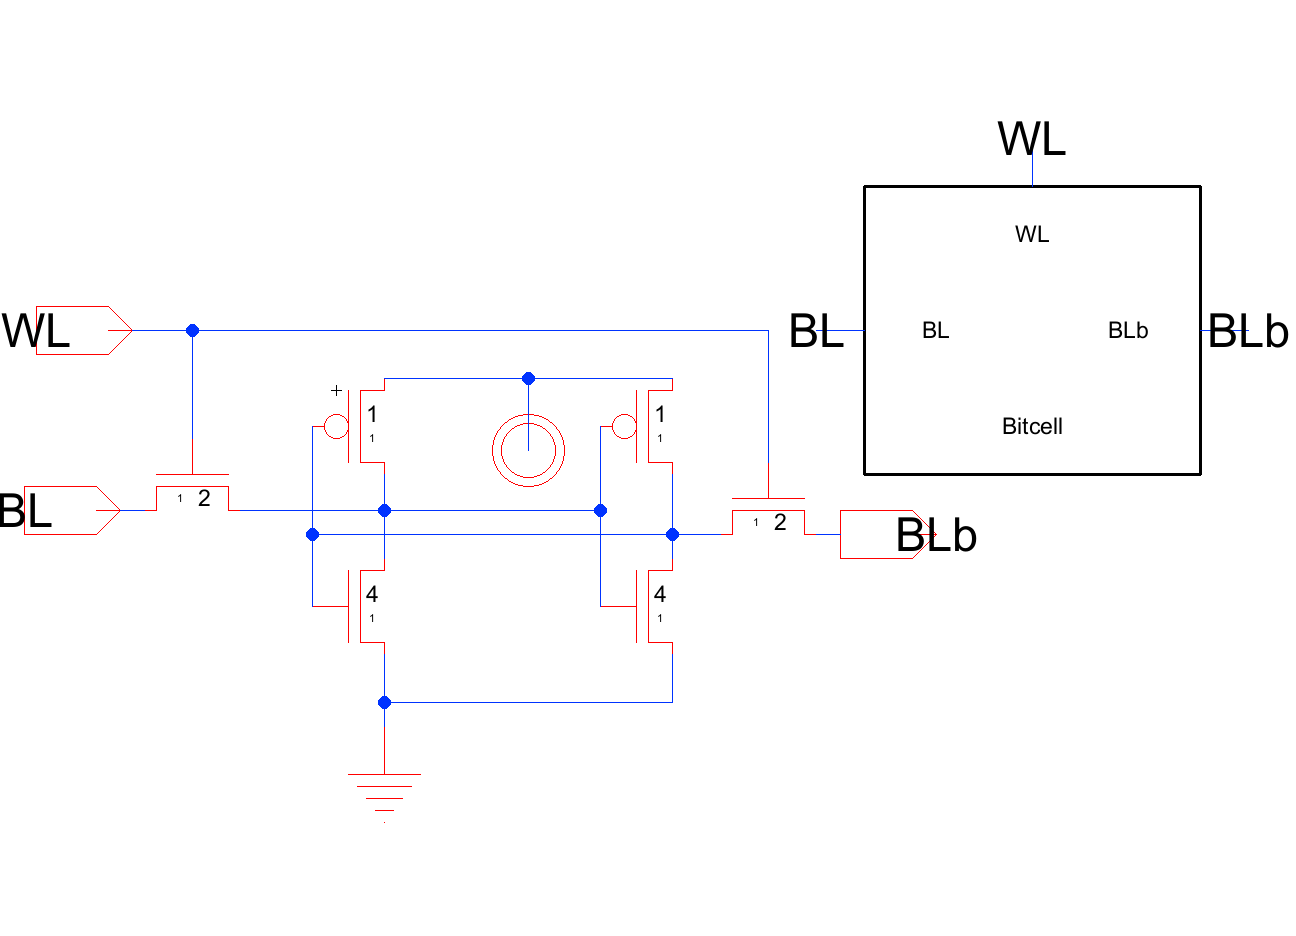
\includegraphics[width=0.45\linewidth]{Bitcell.png}
  \caption{6T SRAM bitcell. Width ratio PD:AX:PU $= 4:2:1$
    (88\,nm\,:\,44\,nm\,:\,22\,nm).}
  \label{fig:bitcell}
\end{figure}

The storage cell is the standard six-transistor SRAM bitcell: a pair of
cross-coupled CMOS inverters and two NMOS access transistors. Width ratios
were chosen to satisfy the two competing static constraints:

\begin{description}
  \item[Read stability.] During a read the access transistor must not allow
    the precharged high bitline to flip the internal low node. This requires
    the pulldown NMOS to be strong relative to the access NMOS (the
    ``cell ratio'' or $\beta_r$). With PD\,:\,AX = $88:44 = 2$, the low node
    rises only a few tens of millivolts during access -- well below the
    inverter trip point.
  \item[Write-ability.] During a write the access transistor must be able to
    pull the internal high node below the inverter trip point against the
    pullup PMOS. This requires the pullup PMOS to be \emph{weak} relative to
    the access NMOS (the ``pullup ratio''). With PU\,:\,AX = $22:44 = 0.5$,
    the access device wins cleanly.
\end{description}

Combined, the absolute ratio PD\,:\,AX\,:\,PU $= 4:2:1$ biases the cell
slightly toward read stability relative to the textbook $2:1:1$ point, which
is a sensible trade-off given that reads happen on every cycle regardless of
\texttt{Wr}. The sum of widths is
\[
  \mathrm{BitcellArea} \;=\; 2(88) + 2(44) + 2(22) \;=\; 308\,\text{nm}
  \;=\; 0.308\um,
\]
which is the quantity used in the FOM (Section~\ref{sec:fom}).

% ------------------------------------------------------------
\subsection{Two-Phase Non-Overlapping Clock Generator}
\label{sec:2phase}
% ------------------------------------------------------------

\begin{figure}[H]
  \centering
  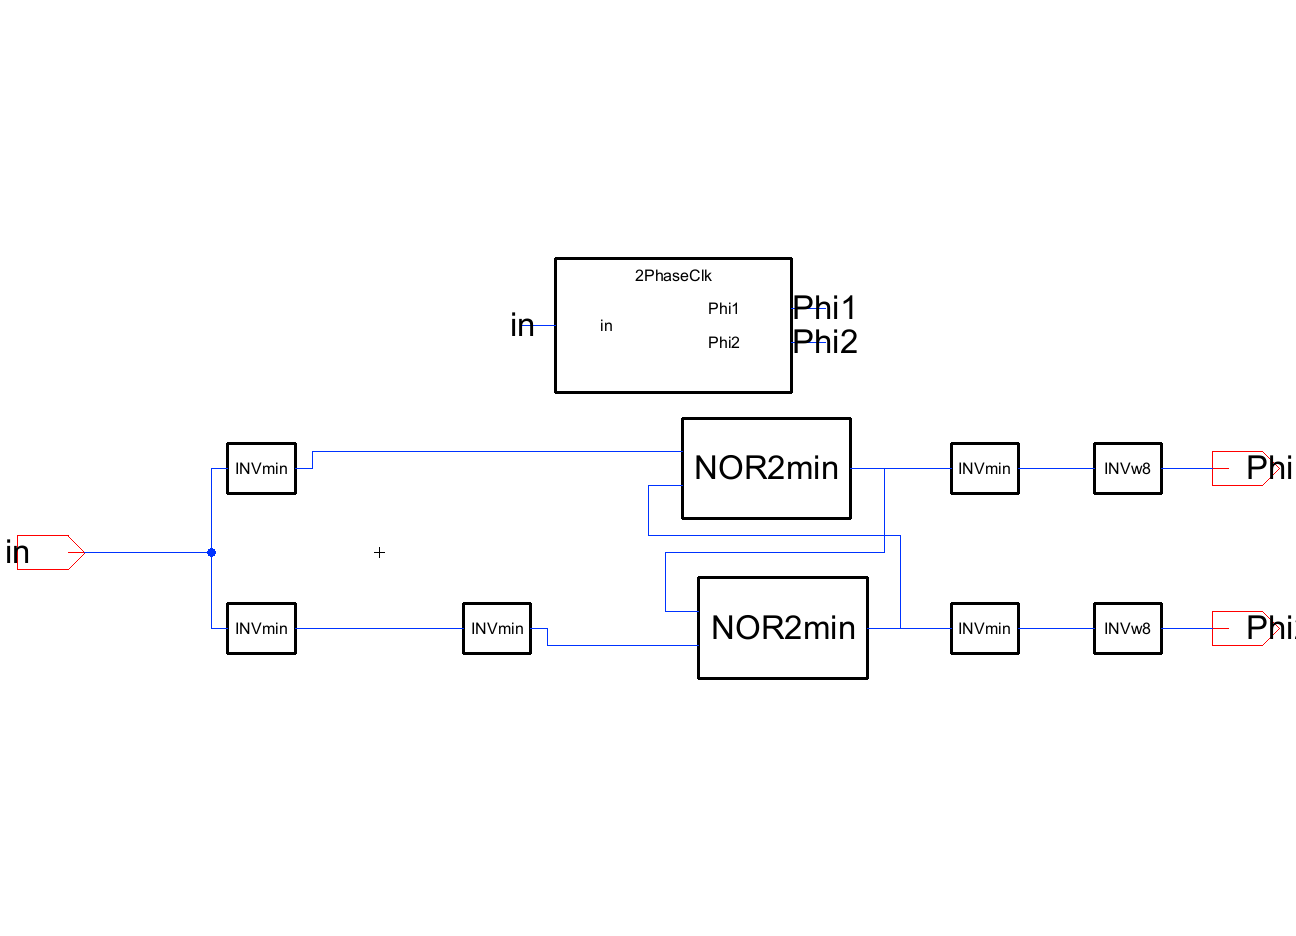
\includegraphics[width=0.70\linewidth]{2PhaseClock.png}
  \caption{Two-phase non-overlapping clock generator. The cross-coupled
    \texttt{NOR2\_min} guarantees that $\phi_1$ and $\phi_2$ are never
    simultaneously high.}
  \label{fig:2phase}
\end{figure}

A single external \texttt{Clk} is converted into two non-overlapping clocks:
$\phi_1$ is the precharge phase and $\phi_2$ is the access phase. The
non-overlap gap between $\phi_1$ falling and $\phi_2$ rising is the entire
reason for using two phases, and is what guarantees that the precharge PMOS
pair is fully off before any word-line rises.

Each output path uses the chain
\texttt{NOR2\_min} $\to$ \texttt{INV\_min} $\to$ \texttt{INV\_sized}
so that the two inverters after the cross-coupled NOR preserve the intended
polarity (a single inverter after the NOR would swap the $\phi_1$/$\phi_2$
labels). The final-stage driver on $\phi_2$ is sized at $W=8\times$ minimum
(\texttt{INV\_w8}, $W_N\approx350$\,nm, $W_P\approx700$\,nm) because it
drives one NAND input per row, or 16 NAND inputs total ($\approx\,$700\,nm
of gate width). The corresponding final-stage driver on $\phi_1$ can remain
minimum because it drives only one downstream inverter (the one that
produces \texttt{PCHb}).

\paragraph{PCHb polarity: \texttt{PCHb}~$=\overline{\phi_1}$, not $\overline{\phi_2}$.}
The precharge control is active-low. The obvious shortcut would be
$\texttt{PCHb} = \phi_2$, which has the correct polarity and needs no extra
gate. That option was rejected: $\phi_2$'s rising edge would simultaneously
turn the precharge PMOS off \emph{and} enable the row NAND that produces WL,
causing brief contention between the still-precharging bitline and the
access path on every read. Deriving \texttt{PCHb} from $\overline{\phi_1}$
instead costs one inverter but lets the non-overlap gap do its job: $\phi_1$
falls, \texttt{PCHb} rises, precharge turns off, and only \emph{after} the
non-overlap gap does $\phi_2$ rise and WL assert. This is the textbook
justification for paying for two clock phases.

% ------------------------------------------------------------
\subsection{4-to-16 Row Decoder}
\label{sec:decoder}
% ------------------------------------------------------------

\begin{figure}[H]
  \centering
  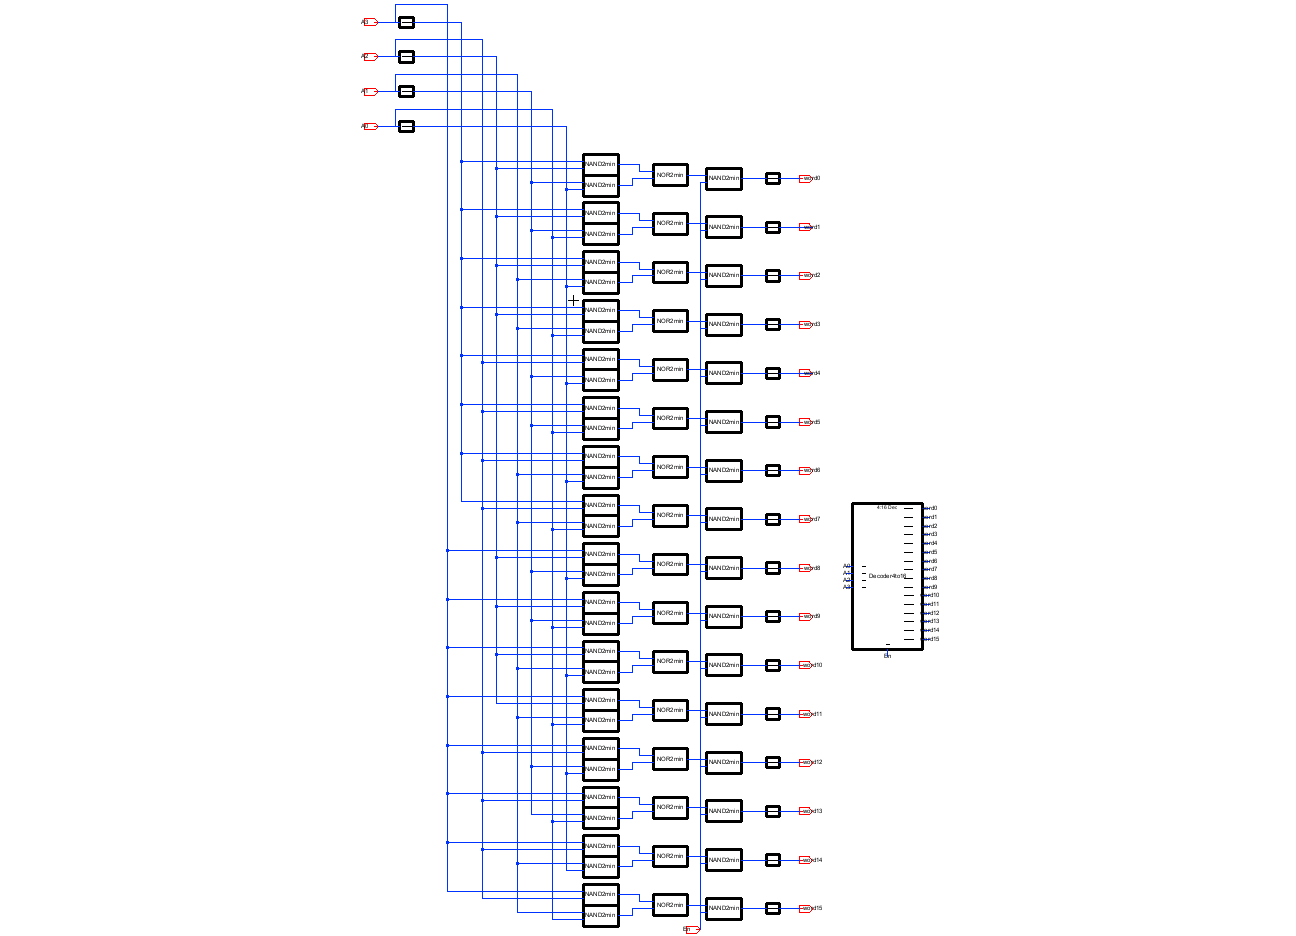
\includegraphics[width=0.85\linewidth]{Decoder4to16.png}
  \caption{4-to-16 row decoder. Each row output is $\mathrm{WL}[i] =
    \mathrm{NAND}(\mathrm{dec}[i],\,\phi_2)$ followed by an inverter, giving
    the required positive-logic, $\phi_2$-gated word-line pulse.}
  \label{fig:decoder}
\end{figure}

The four address bits are decoded through a conventional AND tree into 16
one-hot row lines $\mathrm{dec}[i]$. Each row output is then gated with
$\phi_2$ through a \texttt{NAND2\_min} and an \texttt{INV\_min}, so WL$[i]$
is high only when (a)~the address selects row $i$, and (b)~the SRAM is in
its access phase. The $\phi_2$ gating is what makes changes to the address
during the precharge phase harmless -- WL cannot rise until the next access
phase begins, and the precharge/access invariant (Section~\ref{sec:timing})
keeps the cell contents undisturbed in the interim.

Each WL drives four access-transistor gates (one per column), for roughly
175\,nm of gate capacitance -- easily within the drive of the minimum
inverter that terminates the decoder row.

% ------------------------------------------------------------
\subsection{Column Driver and Precharge}
\label{sec:coldriver}
% ------------------------------------------------------------

\begin{figure}[H]
  \centering
  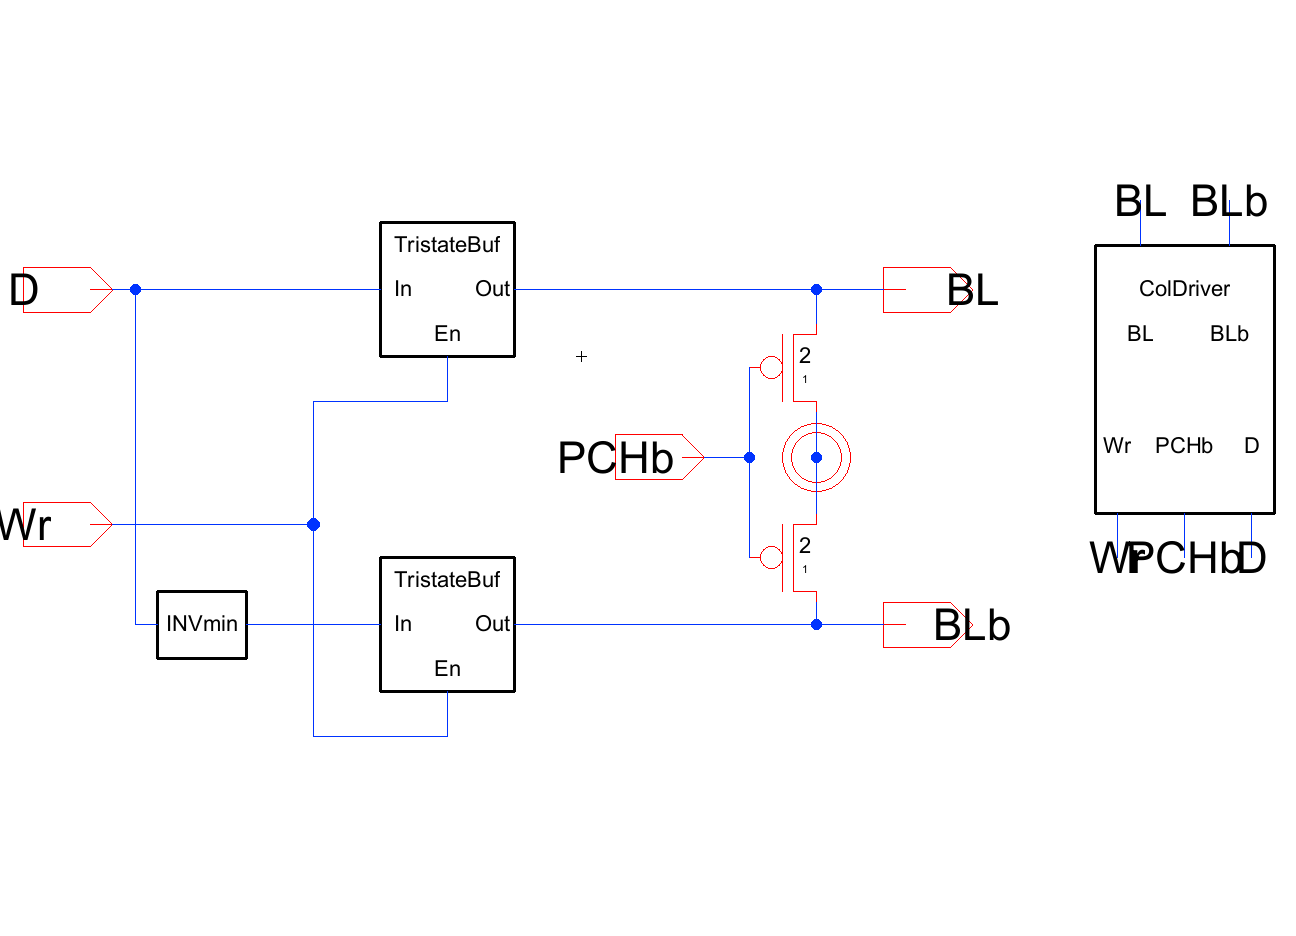
\includegraphics[width=0.72\linewidth]{ColumnDriver.png}
  \caption{One of four identical column drivers. The two PMOS at the top are
    the precharge pair (gated by \texttt{PCHb}); the lower tri-state write
    path (\texttt{RdWr}) drives BL/BLb from the shared bus during write and
    goes high-$Z$ during read.}
  \label{fig:coldriver}
\end{figure}

Each column has two responsibilities that the column driver multiplexes in
time:

\begin{enumerate}
  \item \textbf{Precharge.} Two PMOS, one on BL and one on BLb, are gated by
        \texttt{PCHb}. When \texttt{PCHb} is low, both bitlines are pulled
        to $\Vdd$; when it rises, both PMOS turn off and the bitlines are
        held high by their own capacitance for the duration of the access.
        Each precharge PMOS is sized at $W\approx176$\,nm; the driving
        \texttt{PCHb} inverter (\texttt{INV\_sized}) is sized at
        $W=4\times$ to match the combined 1.4\um\ gate capacitance across
        four columns at roughly FO4.
  \item \textbf{Write.} The write path takes \texttt{bit[i]} from the shared
        bus, drives it onto BL and its complement onto BLb, and tri-states
        when \texttt{Wr} is low. The tri-state is what allows the same BL
        net to be driven by the column driver during write and passively
        observed by the sense amp during read.
\end{enumerate}

No explicit lumped bitline capacitance is added in simulation: the 22\,nm
transistor models already include junction and diffusion capacitance at
source/drain, so adding a parallel \texttt{Cbl} would double-count.

% ------------------------------------------------------------
\subsection{Sense Amplifier}
\label{sec:sa}
% ------------------------------------------------------------

\begin{figure}[H]
  \centering
  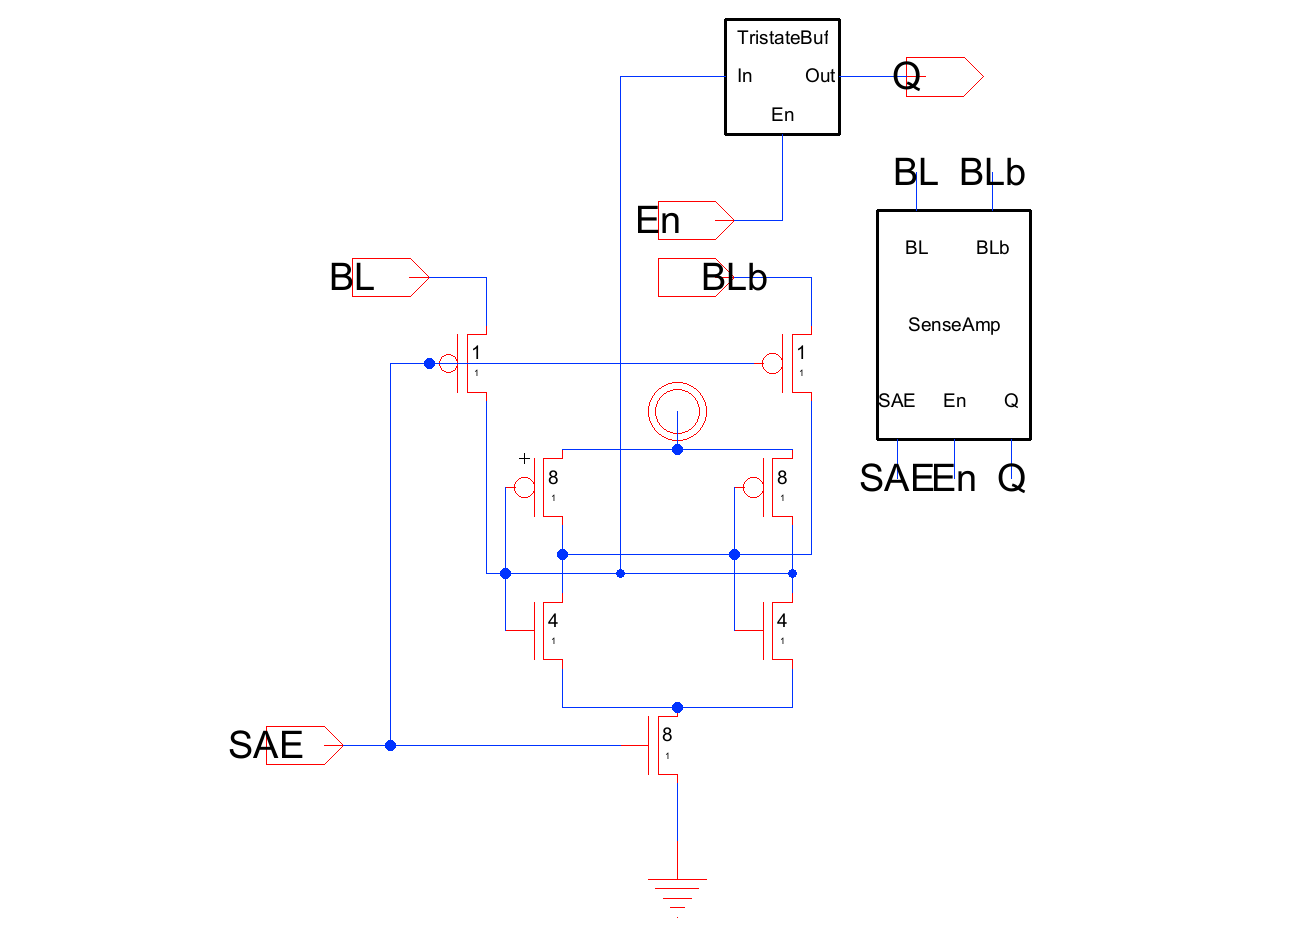
\includegraphics[width=0.60\linewidth]{SenseAmp.png}
  \caption{Isolated latch-type sense amplifier. Cross-coupled CMOS inverter
    pair with two PMOS isolation pass gates between the bitlines and the
    internal latch nodes, and an NMOS footer gated by SAE.
    Topology adapted from~\cite{ra-sa}.}
  \label{fig:sa}
\end{figure}

The sense amplifier is an \emph{isolated} latch-type rather than a plain
bitline-coupled latch. Two PMOS pass transistors, gated by SAE (active-low
from the sense-amp's perspective), connect BL and BLb to the internal latch
nodes during signal development. When SAE rises, the pass PMOS turn off,
isolating the latch from the heavy bitline capacitance, and the NMOS footer
(gated by SAE through the internal \texttt{En}) turns on to fire the latch.
The regeneration then operates on the small internal node capacitance alone,
which is considerably faster and lower-energy than a footer-only latch that
must drag the bitlines through a full transition.

\paragraph{Control gating and output tri-state.} The sense amp is armed only
during read: its \texttt{En} pin is tied to $\nWr$, so the footer is off
during write and the latch cannot be disturbed by the column driver. Its
output, which drives \texttt{bit[i]} on the shared bus, is tri-stated by
$\nWr$ so that the column driver wins the bus during write.

\paragraph{SAE generation.} SAE is produced as
$\mathrm{SAE}=\mathrm{AND}(\phi_{2,\mathrm{delayed}},\,\nWr)$ by an
\texttt{ANDmin} followed by a \texttt{buffer}, with $\phi_{2,\mathrm{delayed}}$
coming from a short chain of \texttt{INV\_min} stages off $\phi_2$. The
target delay from $\phi_2$ rise to SAE rise is 75--100\,ps. At less than
roughly 50\,ps the bitline differential is too small for the sense amp to
resolve reliably; at greater than 100\,ps the bitline has already developed
well past the SA's offset and additional delay is wasted. Measured values
are reported in Section~\ref{sec:rw-waveforms}.

% ------------------------------------------------------------
\subsection{Supporting Cells}
\label{sec:support}
% ------------------------------------------------------------

\begin{table}[H]
  \centering
  \caption{Supporting cells and their canonical sizings.}
  \label{tab:support}
  \begin{tabular}{@{}lllll@{}}
    \toprule
    Cell & $W_N$ (nm) & $W_P$ (nm) & Notes & Used by \\
    \midrule
    \texttt{INV\_min}    & 44  & 88  & minimum & decoder, SAE chain, glue \\
    \texttt{INV\_sized}  & 176 & 350 & $4\times$ min & \texttt{PCHb}, $\nWr$, SAE buffer \\
    \texttt{INV\_w8}     & 350 & 700 & $8\times$ min & $\phi_2$ final driver \\
    \texttt{NAND2\_min}  & 88  & 88  & min        & decoder row gating \\
    \texttt{NOR2\_min}   & 44  & 176 & min        & non-overlap latch \\
    \texttt{buffer}      & --  & --  & two \texttt{INV}s & SAE distribution \\
    \texttt{wordRow}     & --  & --  & composite  & 4 \texttt{Bitcell}s w/ shared WL \\
    \texttt{TristateBuf} / \texttt{RdWr} & --  & --  & composite & write enable path \\
    \bottomrule
  \end{tabular}
\end{table}

% ============================================================
\section{Timing Requirements for Correct Operation}
\label{sec:timing}
% ============================================================

\begin{figure}[H]
  \centering
  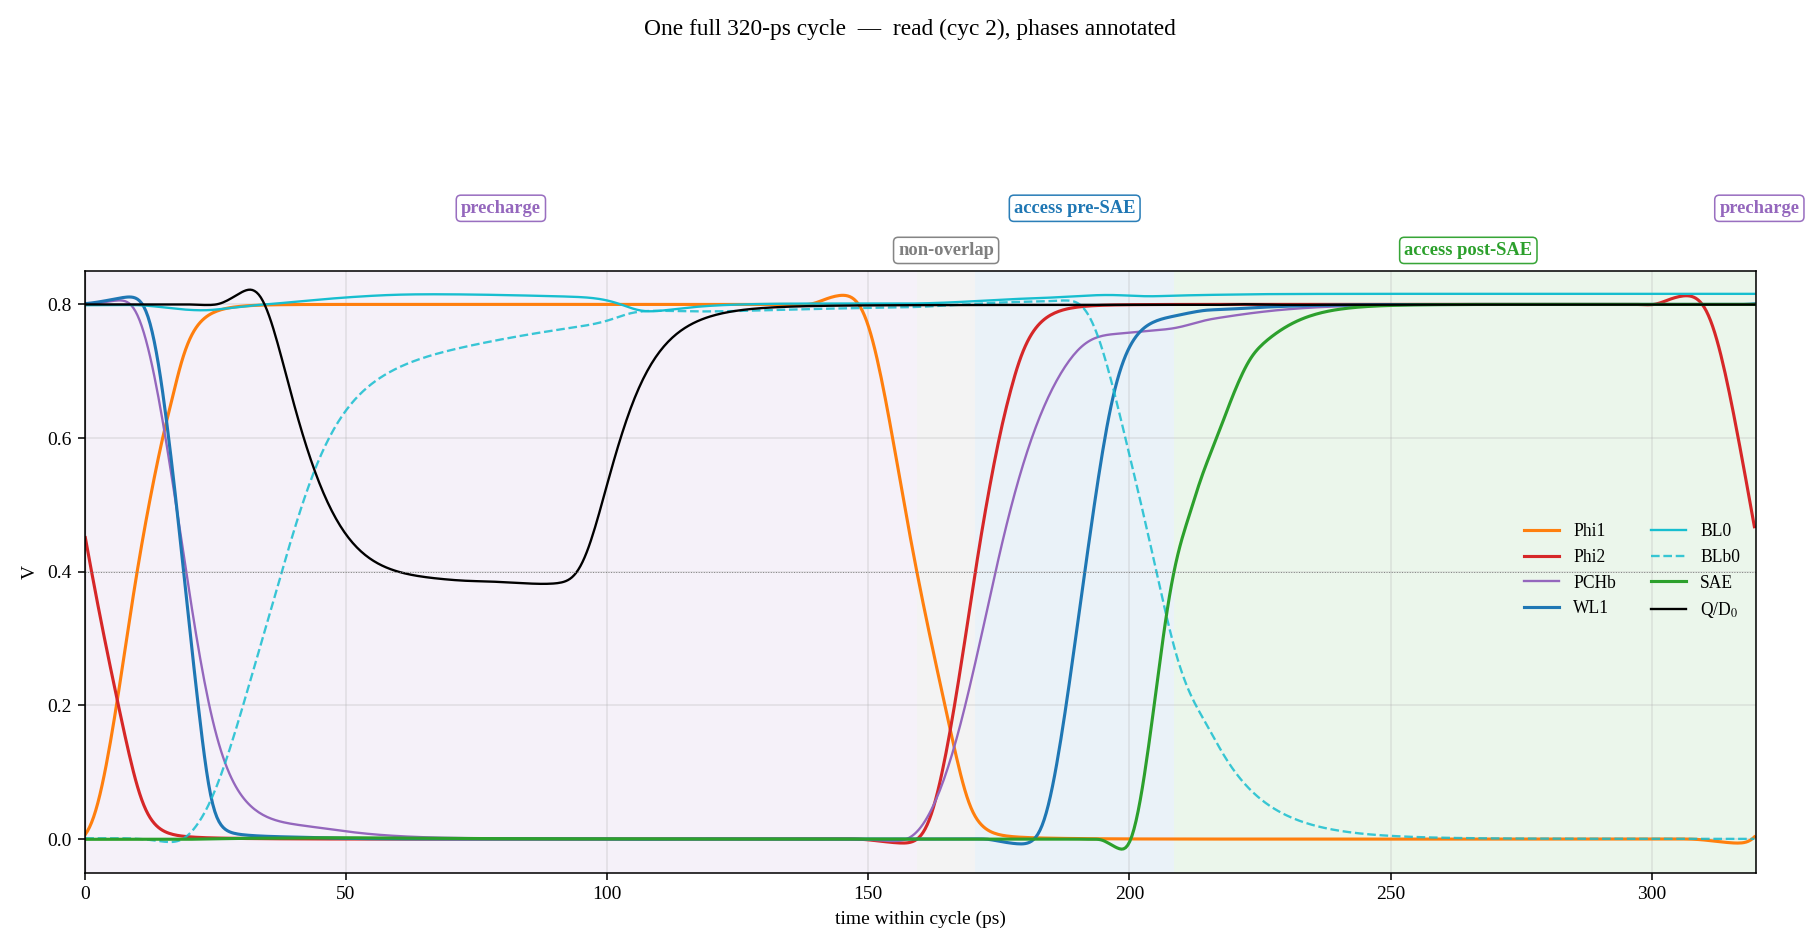
\includegraphics[width=0.95\linewidth]{full_period_320ps.png}
  \caption{One 320\,ps clock period showing the four phases -- precharge,
    non-overlap gap, access pre-SAE, access post-SAE -- overlaid with
    $\phi_1$, $\phi_2$, \texttt{PCHb}, WL, BL/BLb, SAE, and the internal
    sense-amp output $Q$.}
  \label{fig:fullperiod}
\end{figure}

Correct read and write operation is guaranteed by six invariants, each of
which corresponds to a specific ordering of rising and falling edges inside
one clock cycle:

\begin{enumerate}
  \item \textbf{Precharge completes before WL rises.} Ensured because
        \texttt{PCHb}~$=\overline{\phi_1}$ rises with the falling edge of
        $\phi_1$, and WL depends on $\phi_2$, which rises only \emph{after}
        the non-overlap gap.
  \item \textbf{WL rises before SAE fires.} Ensured because SAE goes through
        the \texttt{INV\_min} delay chain off $\phi_2$ (target 75--100\,ps),
        while WL goes through only a \texttt{NAND2}+\texttt{INV}
        (approximately 20\,ps -- see $t_2$ in Table~\ref{tab:read-path}).
  \item \textbf{SAE fires after the bitline has developed beyond the SA's
        offset.} Ensured by tuning the SAE delay so the bitline differential
        at SAE rise exceeds 50\,mV (Table~\ref{tab:read-path},
        $t_3$ to $t_4$).
  \item \textbf{SAE falls before the next precharge begins.} Automatic:
        SAE follows $\phi_2$ and is further gated by $\nWr$.
  \item \textbf{Write driver is tri-stated during read.} Enforced by the
        column driver's internal $\mathtt{Wr}$ gate.
  \item \textbf{Sense-amp output is tri-stated during write.} Enforced by
        the SA's output $\nWr$ gate; also its footer is disabled so the
        latch cannot fight the column driver on BL/BLb.
\end{enumerate}

These six conditions are all satisfied for any non-overlap gap greater than
the worst-case precharge-off delay, any SAE delay greater than the bitline
development time to 50\,mV, and any clock period greater than $T_{\min}$.
The measurement in Section~\ref{sec:tmin} demonstrates that
$T_{\min}=298$\,ps.

% ============================================================
\section{Read and Write Operations with Critical Path}
\label{sec:rw-waveforms}
% ============================================================

The critical path for both operations is the access-phase chain from the
rising edge of $\phi_2$ to either the output driver reaching $\Vdd/2$ (read)
or the cell's internal storage node reaching $\Vdd/2$ (write). The
waveforms below are from \texttt{probed\_320ps\_v2.spi}, an ngspice transient
of the full SRAM driven by the \texttt{mainTest1} stimulus sequence
(\texttt{WR~1111} $\to$ \texttt{RD~1111} $\to$ \texttt{WR~0000} $\to$
\texttt{RD~0000} at address~1). The write endpoint is measured on the
internal bitcell node \texttt{Xmain@0.Xarray@0.XwordRow@14.XBitcell@0.net@35}
rather than on a bitline, because the bitline can reach its final value
before the cross-coupled pair has actually latched. Defining write-complete
at the bitline would systematically under-report the true access time.

% ------------------------------------------------------------
\subsection{Read Operation}
% ------------------------------------------------------------

\begin{figure}[H]
  \centering
  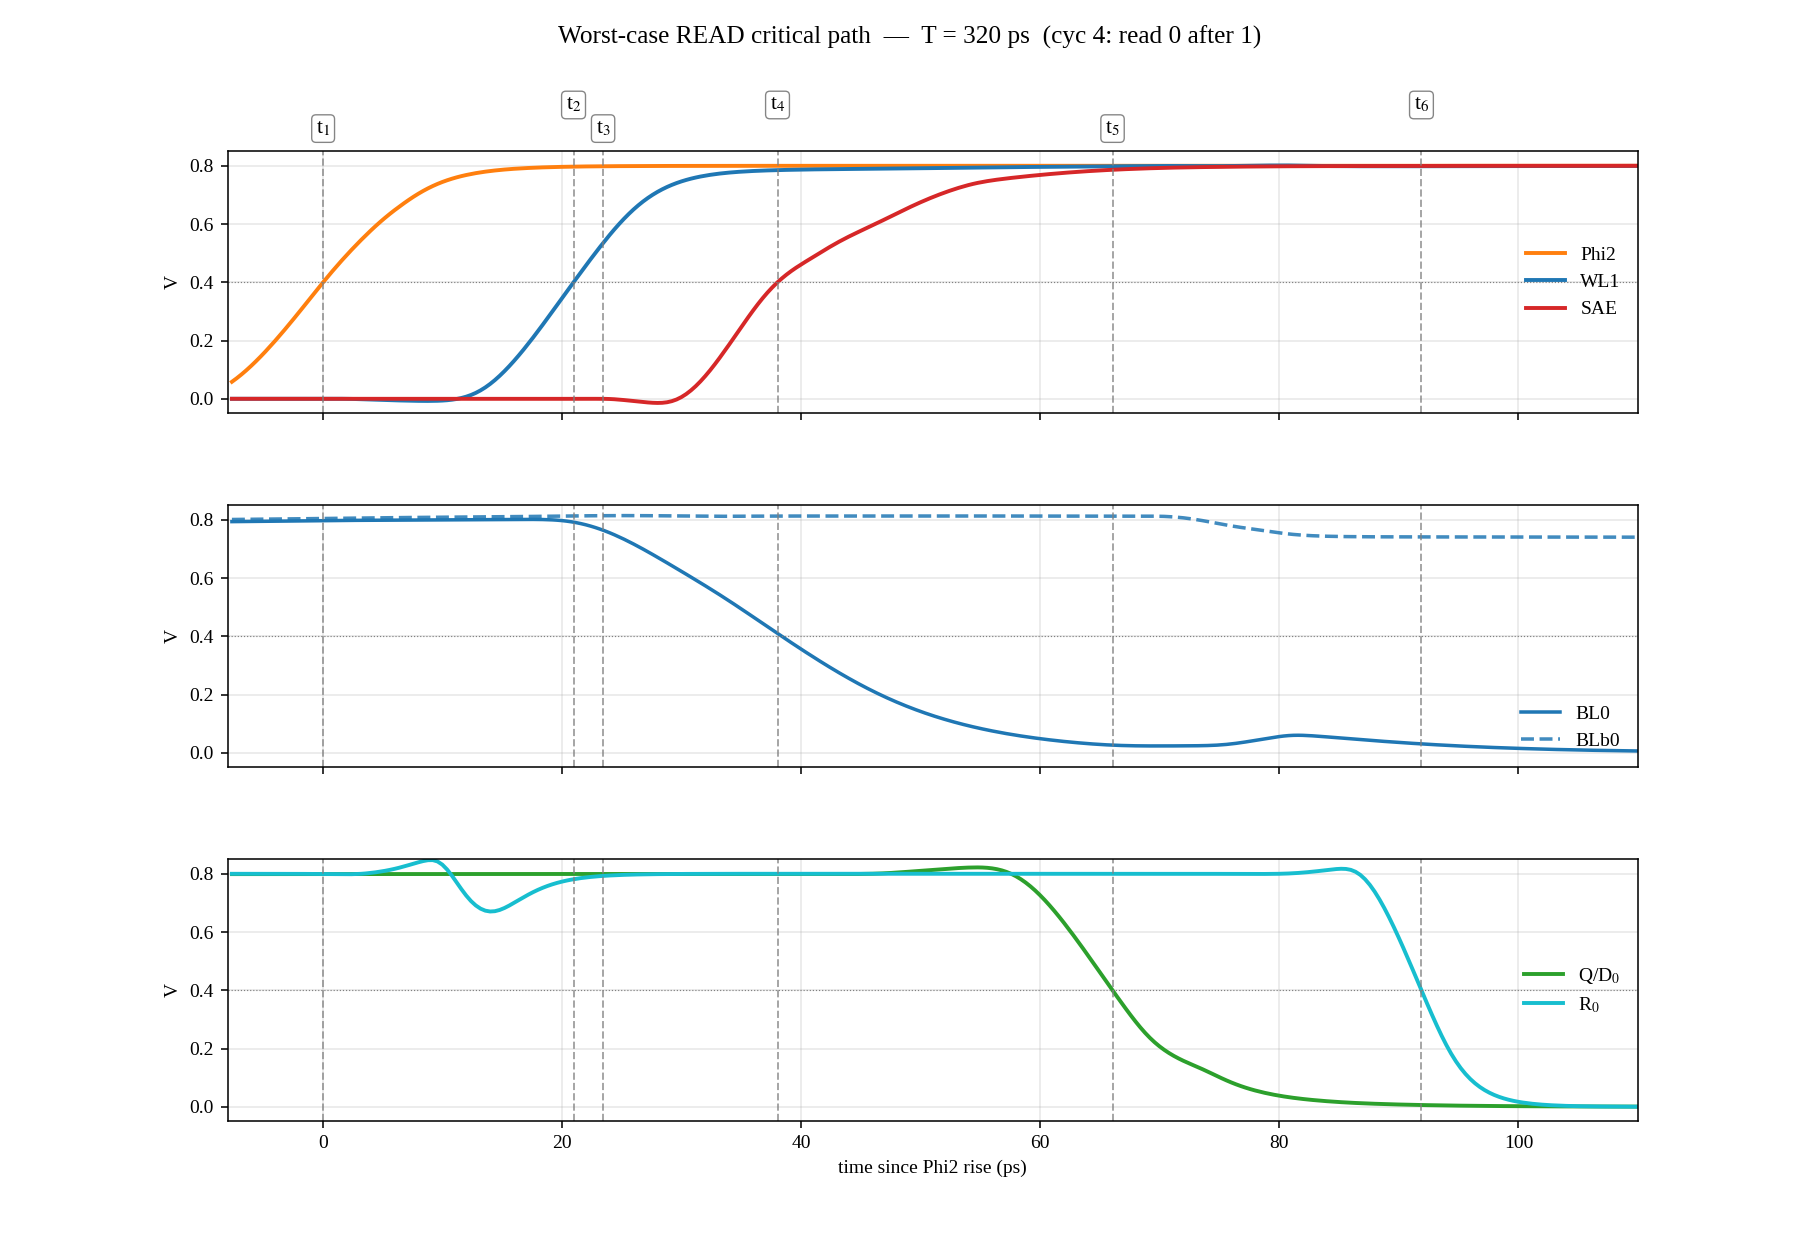
\includegraphics[width=0.95\linewidth]{../figures/breakdown/worst_case_read_zoom.png}
  \caption{Worst-case read (cycle~4: read~0 after previously written~1).
    Markers $t_1\ldots t_6$ correspond to the stages in
    Table~\ref{tab:read-path}.}
  \label{fig:readzoom}
\end{figure}

\begin{table}[H]
  \centering
  \caption{Read critical-path breakdown at $T=320$\,ps. Offsets are from
    the rising edge of $\phi_2$. Threshold convention: $\Vdd/2=0.4$\,V for
    logic edges, 50\,mV for bitline differential.}
  \label{tab:read-path}
  \begin{tabular}{@{}cllc@{}}
    \toprule
    Mark & Offset (ps) & Event & Stage delay (ps) \\
    \midrule
    $t_1$ & 0.0   & $\phi_2$ rises -- access begins                 & --   \\
    $t_2$ & 20.9  & WL1 rises -- decoder NAND+INV propagation done  & 20.9 \\
    $t_3$ & 23.4  & BL differential reaches 50\,mV                  & 2.5  \\
    $t_4$ & 38.0  & SAE fires -- SA armed                           & 14.6 \\
    $t_5$ & 66.0  & $Q/D_0$ at $\Vdd/2$ -- SA resolved              & 28.0 \\
    $t_6$ & \textbf{91.9} & $R_0$ at $\Vdd/2$ -- read latched       & 25.9 \\
    \bottomrule
  \end{tabular}
\end{table}

Total worst-case read delay: $\mathbf{D_{\text{read}} = 91.9\,\text{ps}}$.

% ------------------------------------------------------------
\subsection{Write Operation}
% ------------------------------------------------------------

\begin{figure}[H]
  \centering
  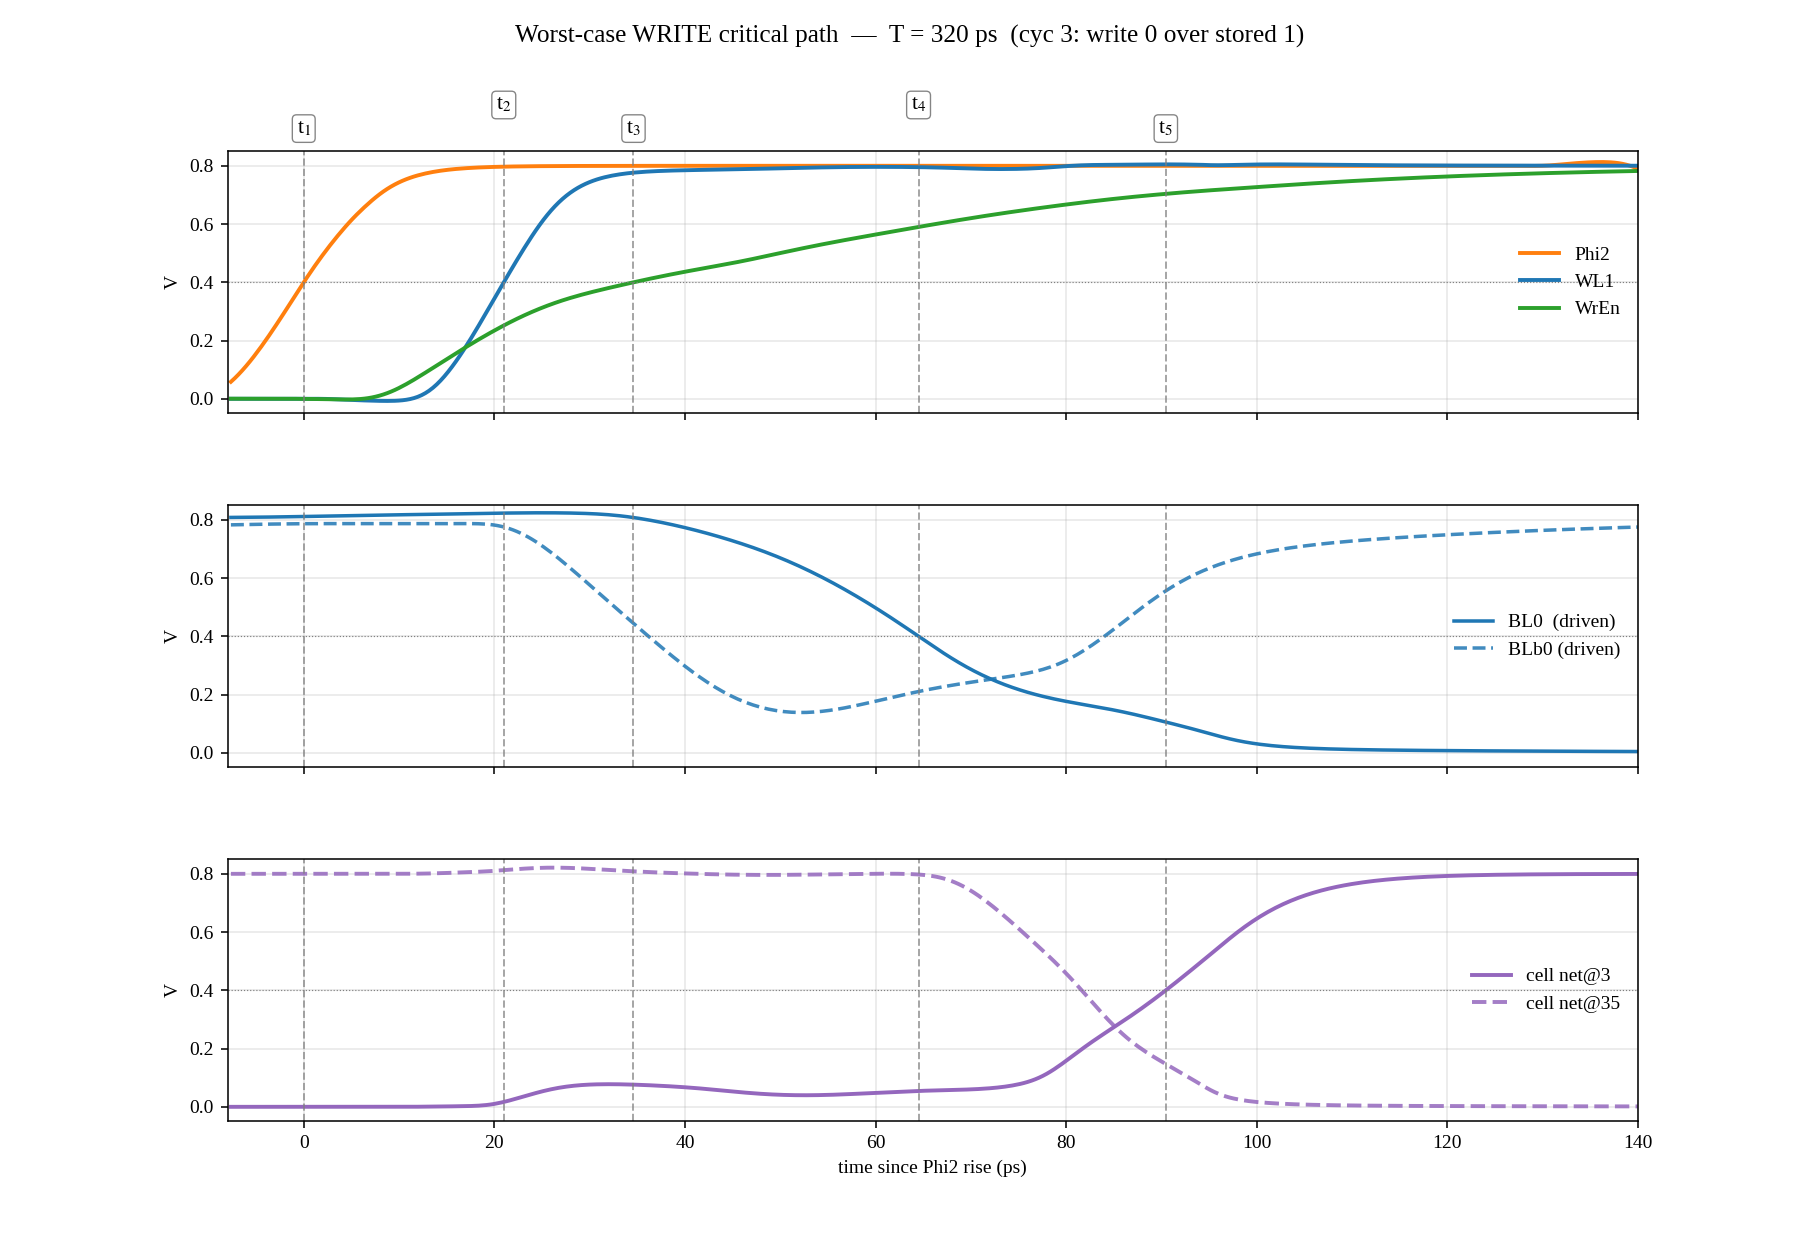
\includegraphics[width=0.95\linewidth]{../figures/breakdown/worst_case_write_zoom.png}
  \caption{Worst-case write (cycle~3: write~0 over a previously stored~1).
    Markers $t_1\ldots t_5$ correspond to the stages in
    Table~\ref{tab:write-path}.}
  \label{fig:writezoom}
\end{figure}

\begin{table}[H]
  \centering
  \caption{Write critical-path breakdown at $T=320$\,ps.}
  \label{tab:write-path}
  \begin{tabular}{@{}cllc@{}}
    \toprule
    Mark & Offset (ps) & Event & Stage delay (ps) \\
    \midrule
    $t_1$ & 0.0   & $\phi_2$ rises -- access begins               & --   \\
    $t_2$ & 21.0  & WL1 rises                                     & 21.0 \\
    $t_3$ & 34.6  & WrEn rises -- column drivers enabled          & 13.6 \\
    $t_4$ & 64.5  & BL0 crosses $\Vdd/2$ -- data on bitline       & 29.9 \\
    $t_5$ & \textbf{90.5} & Cell internal node at $\Vdd/2$ -- write committed & 26.0 \\
    \bottomrule
  \end{tabular}
\end{table}

Total worst-case write delay: $\mathbf{D_{\text{write}} = 90.5\,\text{ps}}$.

\paragraph{Worst-case delay (reported).}
$D = \max(D_{\text{read}}, D_{\text{write}}) = 91.9$\,ps.

% ============================================================
\section{Design Validation and Test Cases}
\label{sec:validation}
% ============================================================

Correctness was validated bottom-up, starting from the bitcell and moving
outward.

% ------------------------------------------------------------
\subsection{Bitcell Unit Test}
% ------------------------------------------------------------

\begin{figure}[H]
  \centering
  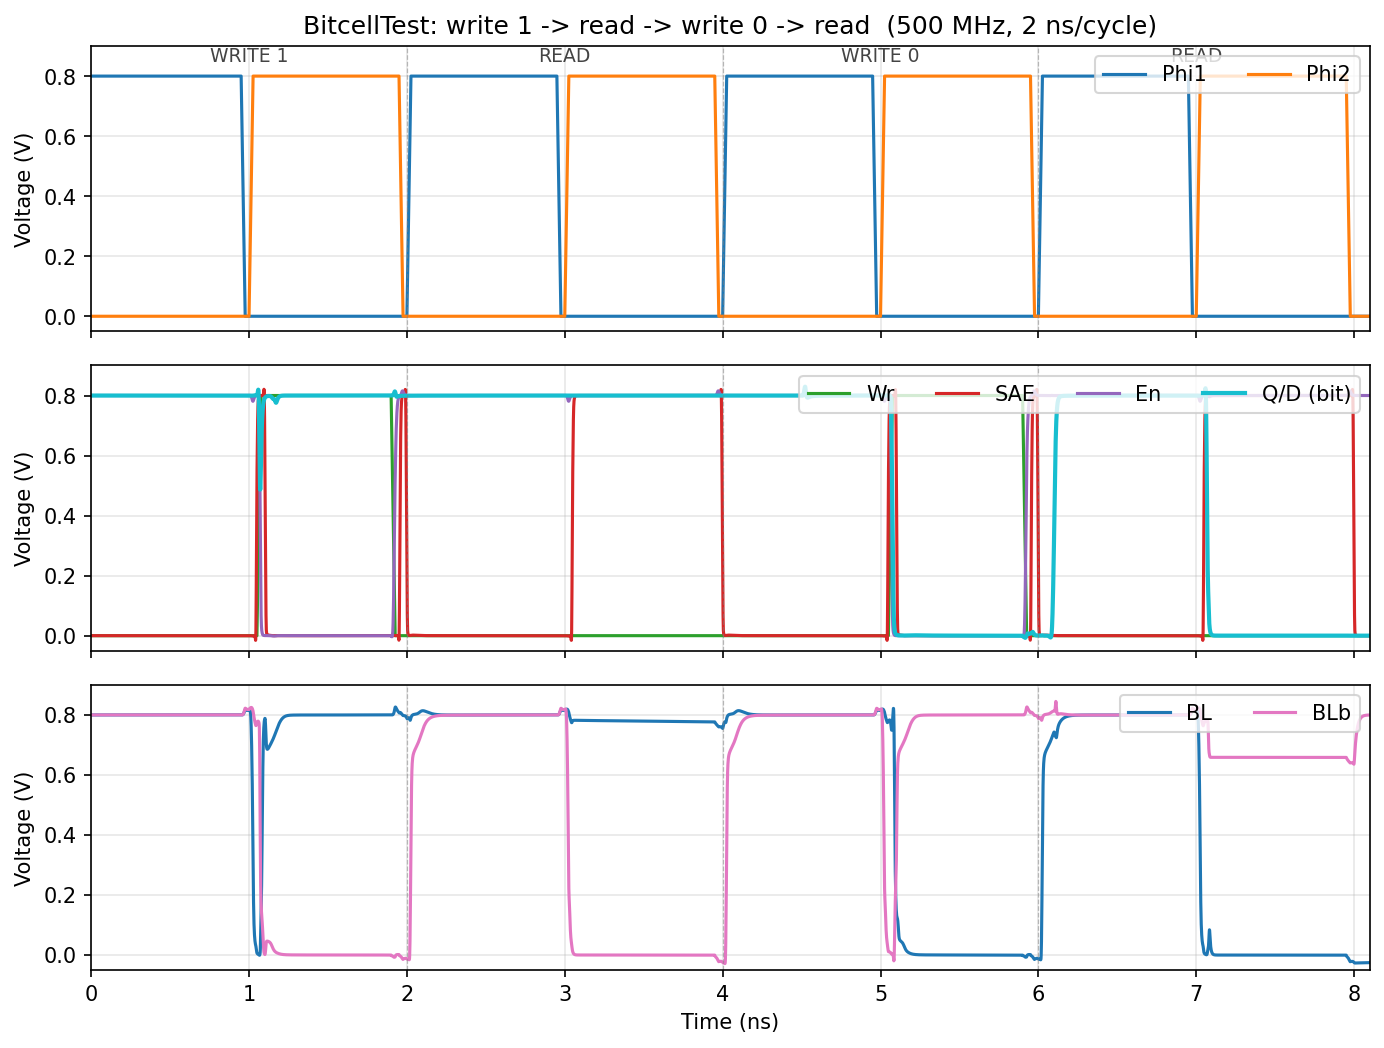
\includegraphics[width=0.92\linewidth]{BitcellTest_waveforms.png}
  \caption{Bitcell unit test. A single cell is exercised by a PWL stimulus
    covering write~0, write~1, and a non-destructive read of each polarity.
    The internal storage nodes $Q$ and $\overline{Q}$ track the written
    value and remain stable during the subsequent read.}
  \label{fig:bitcelltest}
\end{figure}

The bitcell test covers the two independent correctness conditions:
\emph{write ability} (the cell can be flipped in both directions) and
\emph{read stability} (the cell survives a read in both polarities without
disturbing the stored value). Both conditions are met for the chosen
$4:2:1$ sizing.

% ------------------------------------------------------------
\subsection{Full-Array Functional Test (\texttt{mainTest1})}
% ------------------------------------------------------------

\begin{figure}[H]
  \centering
  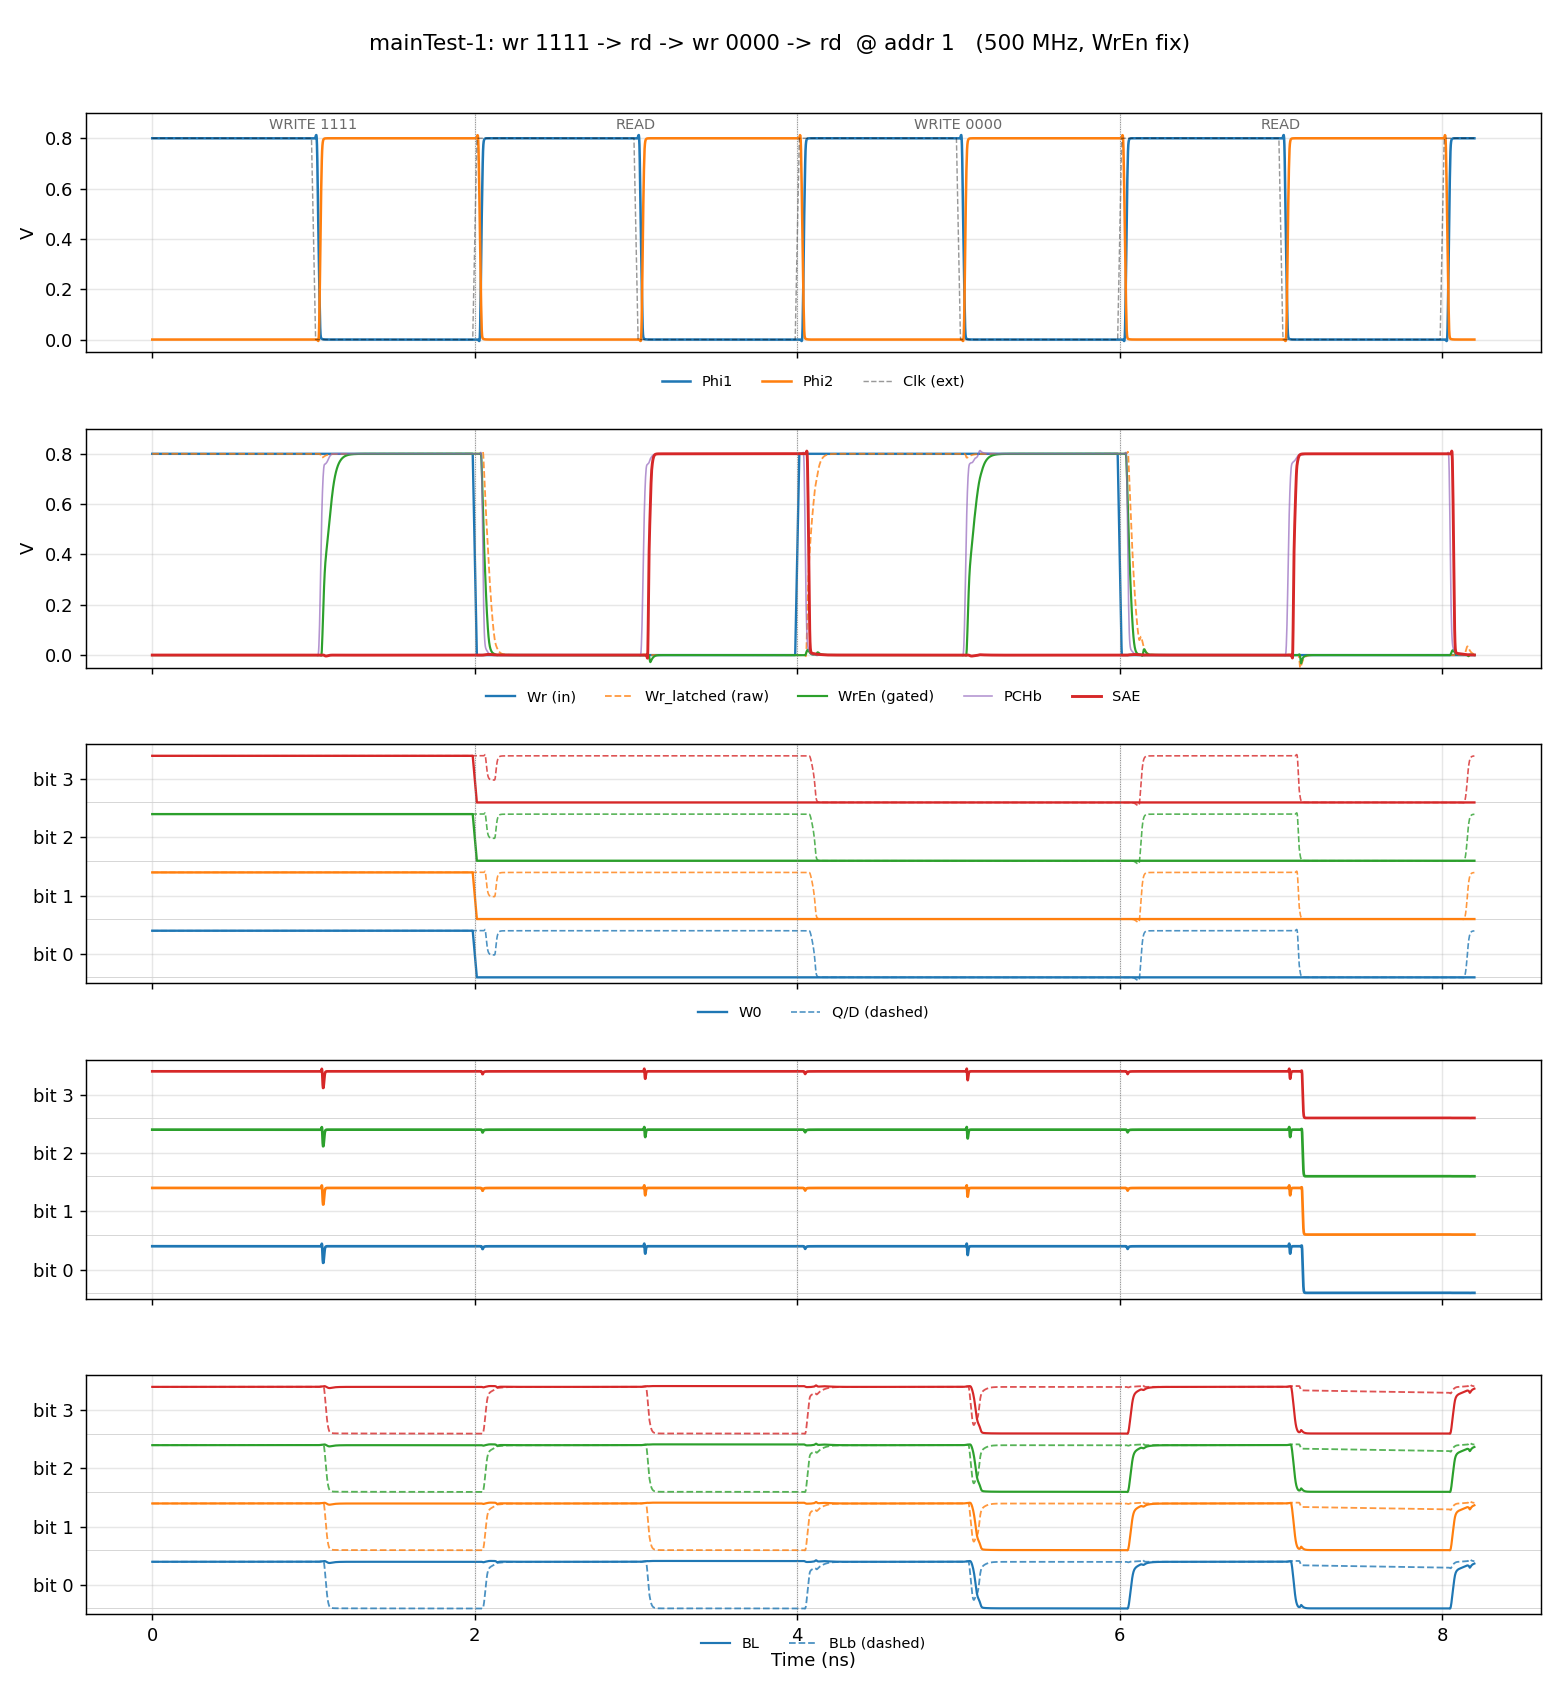
\includegraphics[width=0.98\linewidth]{mainTest1_waveforms.png}
  \caption{\texttt{mainTest1} -- full SRAM stimulus exercising write~1,
    read~1, write~0, read~0 at a single address across four cycles. All
    four read outputs match the previously written values.}
  \label{fig:main1}
\end{figure}

% ------------------------------------------------------------
\subsection{Hard-Direction Full-Array Stress (\texttt{mainTest2})}
% ------------------------------------------------------------

\begin{figure}[H]
  \centering
  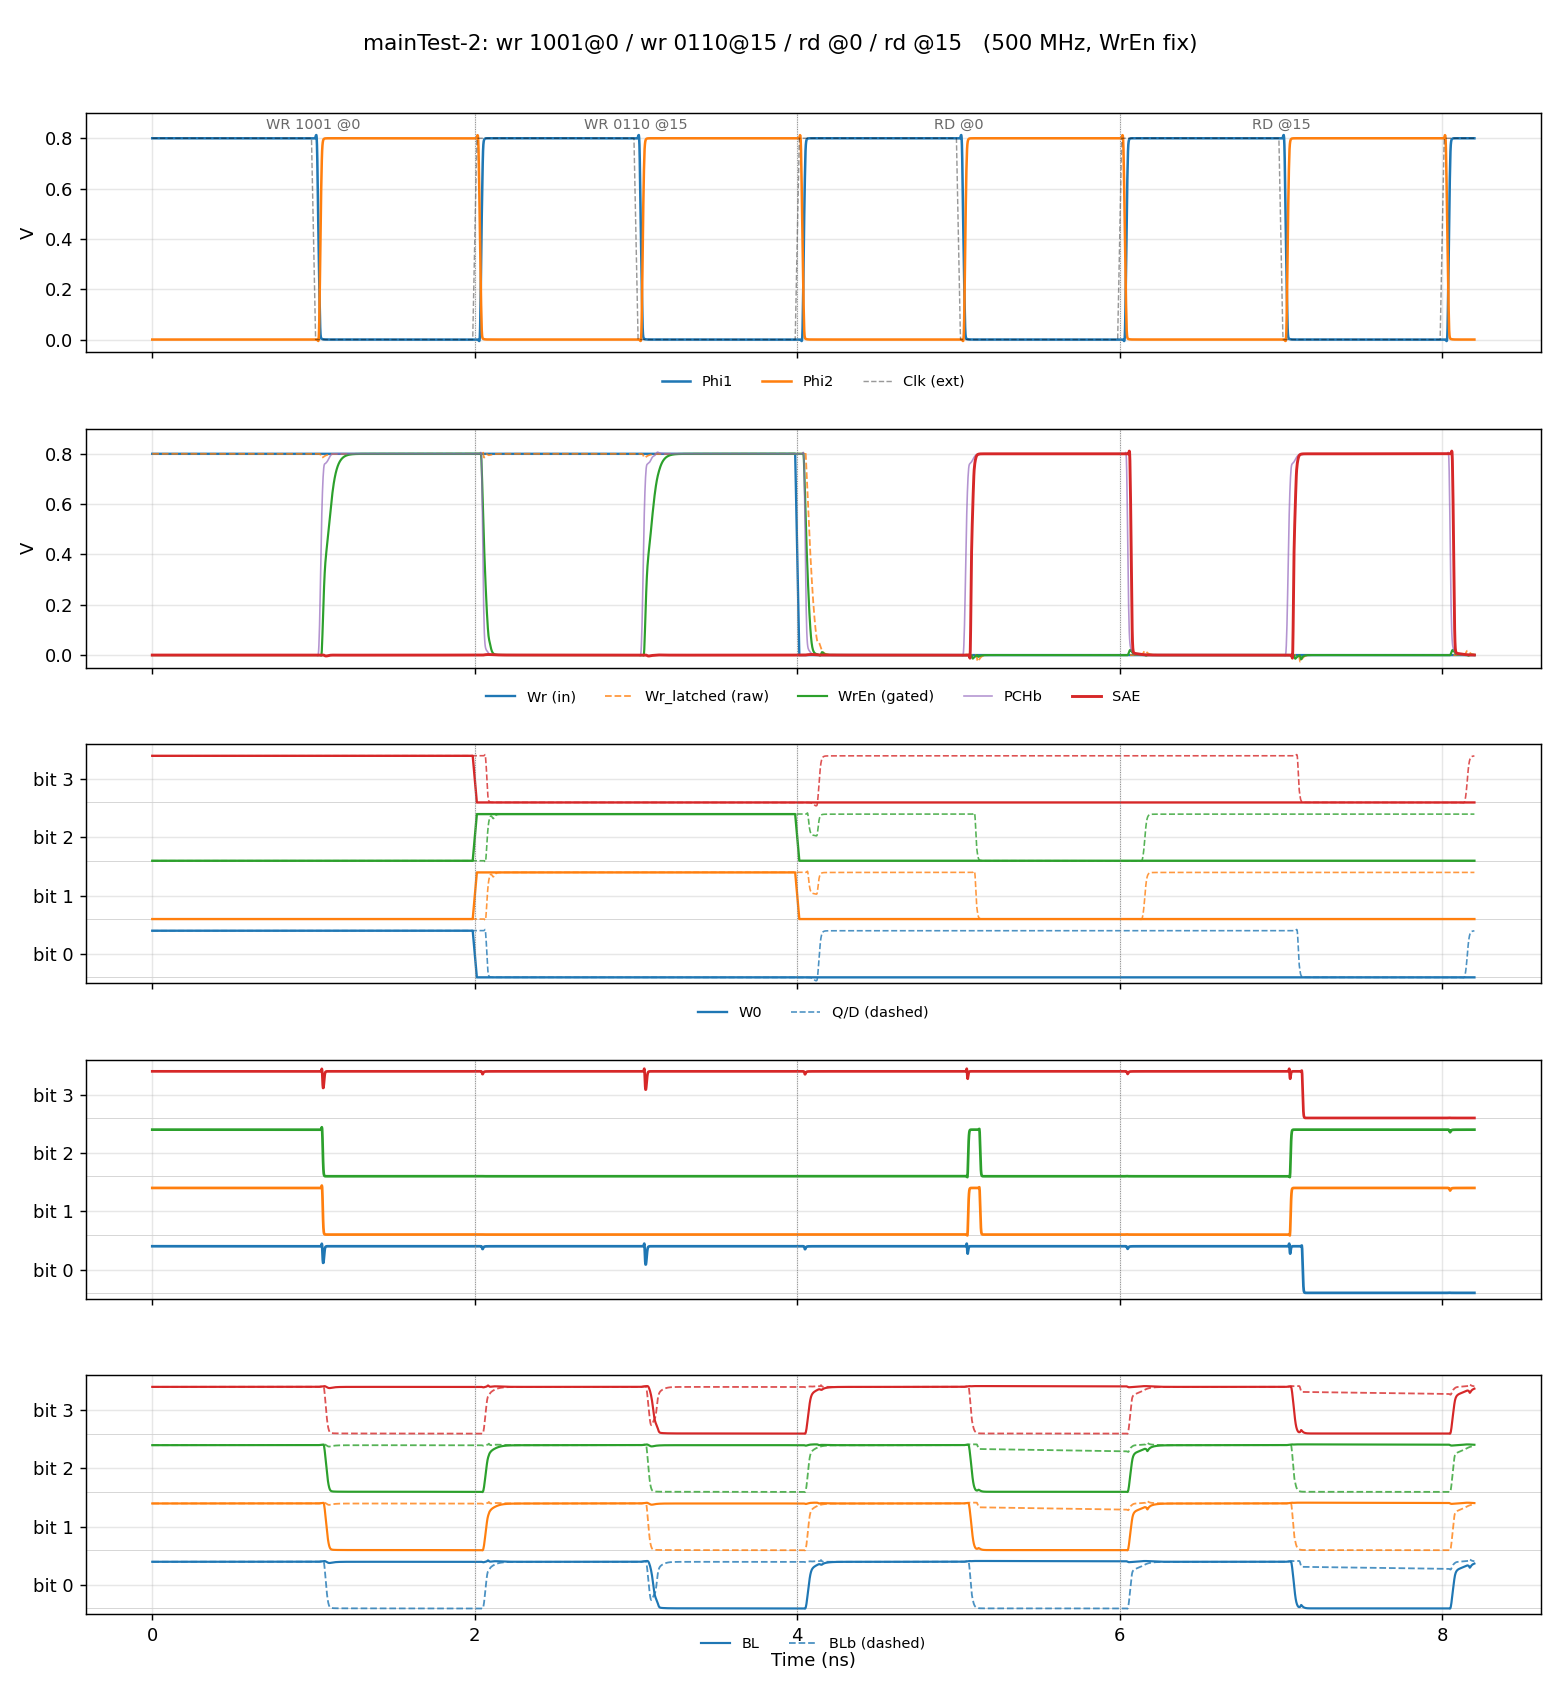
\includegraphics[width=0.98\linewidth]{mainTest2_waveforms.png}
  \caption{\texttt{mainTest2} -- fill the entire array with 1s, fill with
    0s, then read every location. This is the FOM power workload and also
    the stress test that sets $T_{\min}$.}
  \label{fig:main2}
\end{figure}

% ------------------------------------------------------------
\subsection{Test-Case Coverage}
% ------------------------------------------------------------

The test suite exercises the following cases, which together cover every
functional pathway of the design:

\begin{itemize}
  \item \textbf{Write/read both polarities at one address} --
        \texttt{mainTest1}; detects any gross write-path or read-path
        malfunction.
  \item \textbf{Full-array write-0s / write-1s} -- \texttt{mainTest2};
        stresses the decoder across all 16 rows and confirms the address
        path.
  \item \textbf{Read-after-write at each address} -- implicit in
        \texttt{mainTest2}; the read pass after the all-0s and all-1s
        writes verifies that the entire array holds the written values.
  \item \textbf{Worst-direction transitions} -- write~0 over stored~1 and
        read~0 after stored~1 are the slowest operations in each category
        (the SA starts with the precharged-high BL assisting a read~1 but
        fighting a read~0, and the column driver must pull BL from $\Vdd$
        to ground for a write~0). These are the cycles plotted in
        Section~\ref{sec:rw-waveforms}.
\end{itemize}

% ============================================================
\section{Performance Characterization}
% ============================================================

% ------------------------------------------------------------
\subsection{Minimum Clock Period}
\label{sec:tmin}
% ------------------------------------------------------------

\begin{figure}[H]
  \centering
  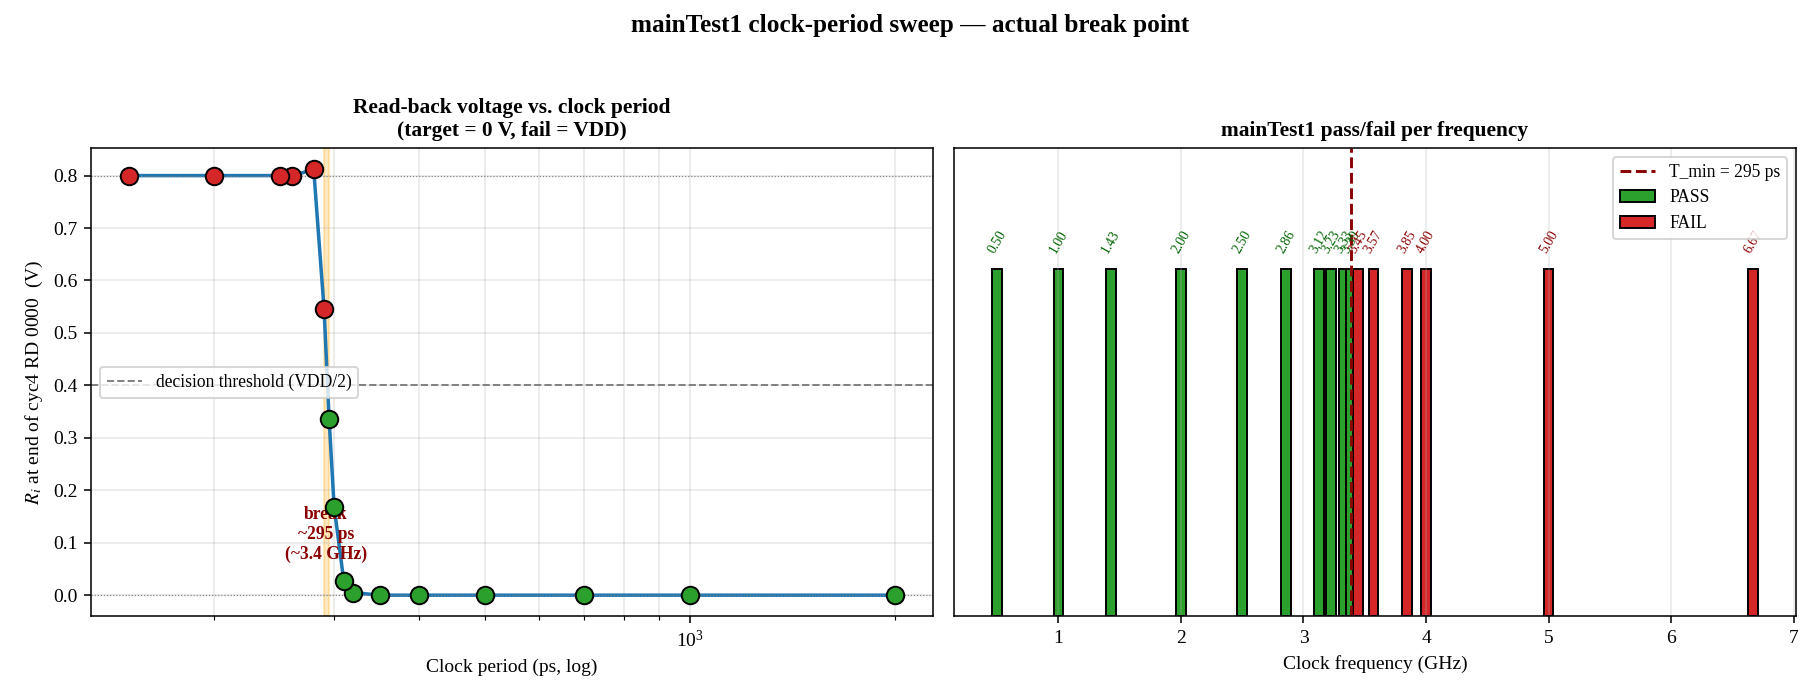
\includegraphics[width=0.90\linewidth]{period_sweep.png}
  \caption{Clock-period sweep on the \texttt{mainTest2} workload.
    $T_{\min}=298$\,ps (296\,ps fails, 298\,ps passes). The measurement
    in Section~\ref{sec:power} uses $T=320$\,ps, roughly 7\% margin above
    $T_{\min}$.}
  \label{fig:sweep}
\end{figure}

The minimum clock period was found by sweeping $T$ downward on the hard
\texttt{mainTest2} workload until a read failed. Below $T\approx 298$\,ps
the array begins to return incorrect data; at $T=298$\,ps every read
passes. The maximum operating frequency is therefore
\[
  f_{\max} = \frac{1}{T_{\min}} = \frac{1}{298\,\text{ps}}
          \approx 3.36\,\text{GHz},
\]
well above the project's 500\,MHz minimum.

At $T_{\min}$ the read path still completes in approximately 91.7\,ps, so
the failure boundary is set by the \emph{write} path (word-line pulse
width and cross-coupled cell flip margin), not by sense-amp resolution.
Adding margin on the write side would close this gap further.

% ------------------------------------------------------------
\subsection{Power Measurement}
\label{sec:power}
% ------------------------------------------------------------

\begin{figure}[H]
  \centering
  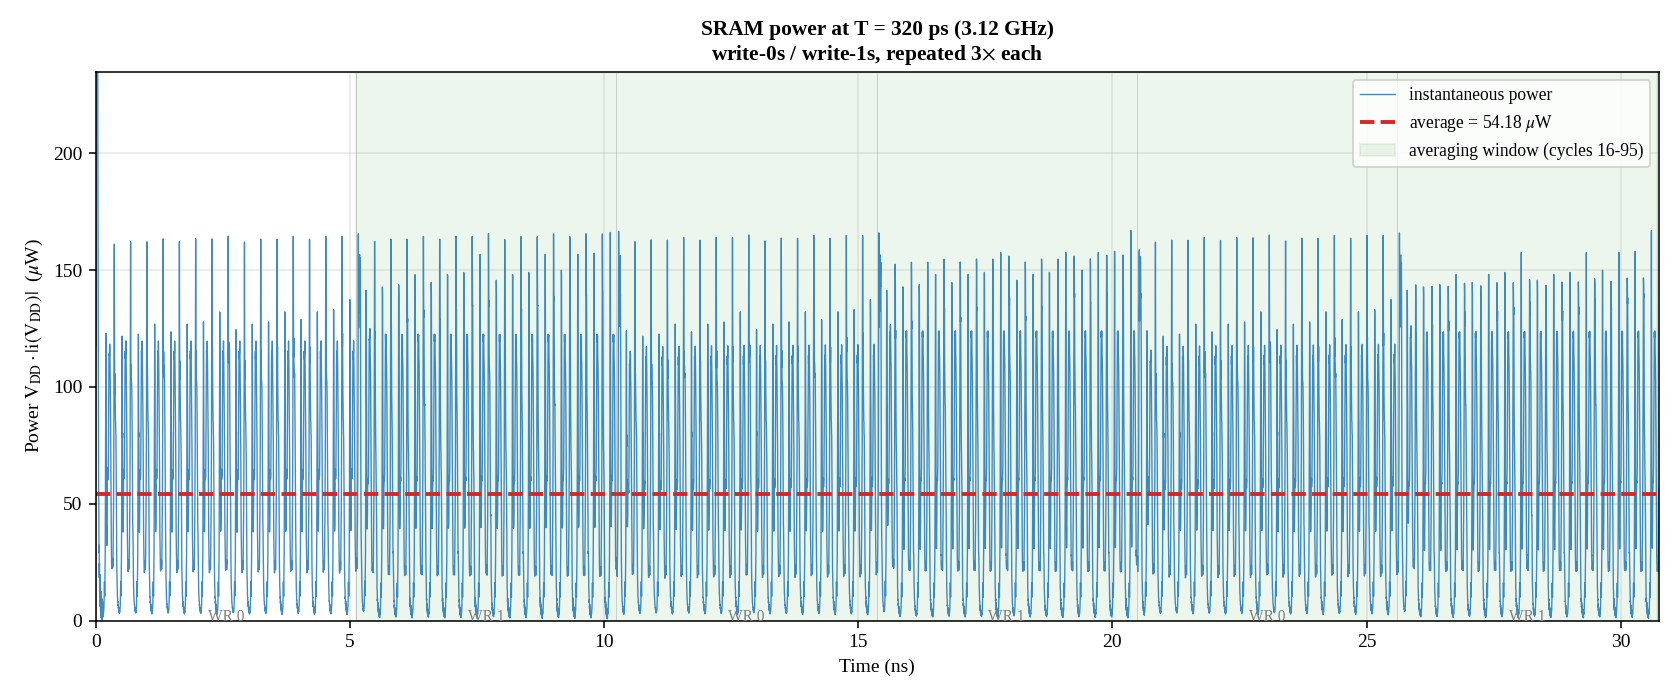
\includegraphics[width=0.95\linewidth]{power_320ps.png}
  \caption{Average supply current at $T=320$\,ps during the FOM workload
    -- four repetitions of (write all-0s, write all-1s). Averaging over
    cycles 16--95 excludes initial transient and gives $P=54.18\uW$.}
  \label{fig:power}
\end{figure}

Per the project specification, average power is measured while repeatedly
writing all-0s and then all-1s to the entire array, with the clock set to
a period just above $T_{\min}$. We use $T=320$\,ps (3.125\,GHz), which
provides $\sim7\%$ margin over $T_{\min}$ and aligns with a clean point on
the period sweep grid. Averaging the supply current over cycles 16--95
(excluding the initial settling transient) gives
\[
  P = 54.18\uW.
\]

% ------------------------------------------------------------
\subsection{Figure of Merit}
\label{sec:fom}
% ------------------------------------------------------------

With the measured inputs
\[
  \mathrm{BitcellArea} = 0.308\um,\qquad
  P = 54.18\uW,\qquad
  D = 91.9\,\text{ps},
\]
the FOM evaluates to
\begin{align*}
  \mathrm{FOM}
  &= 60 \cdot 0.308\um \cdot 54.18\uW \cdot (91.9\,\text{ps})^2 \\
  &= 60 \cdot 0.308 \cdot 54.18 \cdot 8445.61
     \;\mu\text{m}\cdot\mu\text{W}\cdot\text{ps}^{2} \\
  &\approx \mathbf{8.46\times10^{6}\ \mu\text{m}\cdot\mu\text{W}\cdot\text{ps}^{2}}.
\end{align*}

% ------------------------------------------------------------
\subsection{Summary of Metrics}
% ------------------------------------------------------------

\begin{table}[H]
  \centering
  \caption{Summary of design metrics.}
  \label{tab:summary}
  \begin{tabular}{@{}lr@{}}
    \toprule
    Metric & Value \\
    \midrule
    Technology                        & 22\,nm PTM HP \\
    Supply voltage $\Vdd$             & 0.8\,V \\
    Array size                        & $16\times4$ \\
    Bitcell sizing (PD\,:\,AX\,:\,PU) & $88:44:22$\,nm ($4:2:1$) \\
    BitcellArea (sum of widths)       & $0.308\um$ \\
    Minimum clock period $T_{\min}$   & 298\,ps \\
    Maximum clock frequency           & 3.36\,GHz \\
    Measurement period $T$            & 320\,ps (3.125\,GHz) \\
    Worst-case read access time       & 91.9\,ps \\
    Worst-case write access time      & 90.5\,ps \\
    Reported delay $D$                & 91.9\,ps \\
    Average power $P$                 & $54.18\uW$ \\
    \textbf{FOM}                      & $\mathbf{8.46\times10^{6}\ \mu\text{m}\cdot\mu\text{W}\cdot\text{ps}^{2}}$ \\
    \bottomrule
  \end{tabular}
\end{table}

% ============================================================
\section{Conclusion}
% ============================================================

The $16\times4$ SRAM meets all functional and performance targets. The two
largest design decisions -- the two-phase clocking scheme with
$\texttt{PCHb}=\overline{\phi_1}$, and the isolated latch-type sense
amplifier gated by a $\phi_2$-derived SAE -- together ensure a clean
separation between precharge and access phases and enable reliable
sense-amp resolution on a controlled bitline differential. The remaining
margin at $T_{\min}$ is spent on the write path, which is the most
promising target for further optimization.

% ============================================================
% References (thebibliography emits its own heading)
% ============================================================

\begin{thebibliography}{9}
  \bibitem{ra-sa}
  \emph{Latch-type sense amplifier,} ResearchGate, figure 4.\\
  \url{https://www.researchgate.net/figure/Latch-type-sense-amplifier_fig4_2977800}
\end{thebibliography}

% ============================================================
% Academic Integrity Statement
% ============================================================

\vspace{2em}

\noindent
\fbox{\parbox{0.95\linewidth}{%
  I, Lucas Krippendorff, certify that I have complied with the University
  of Pennsylvania's Code of Academic Integrity in completing this project.
}}

\end{document}
